% EF5342 Week 4 — The Money Markets
% Beamer conversion from week4_MoneyMarket.pptx (60 source slides -> 40 frames).
% Compile: pdflatex week4_MoneyMarket.tex
% Each frame carries a [src: ...] comment mapping back to source slides
% (the content-coverage checklist; S = section divider slide in the pptx).
\documentclass[aspectratio=169]{beamer}
\usepackage{../ef5342}

\title{EF5342 Financial Systems, Markets and Instruments}
\subtitle{Week 4 --- The Money Markets}
\author{Prof.\ Weikai Li}
\institute{City University of Hong Kong}
\date{Semester B 2026--2027}

\begin{document}

% ============ THE MONEY MARKETS ============

% [src: 1]
% Title-slide background art (slide01_img.jpg) dropped — decorative.
\begin{frame}
\titlepage
\end{frame}

% [src: 2]
\section{The Money Markets}

% [src: 3]
\begin{frame}{Overview}
We review the money markets and the securities traded there, and discuss why the money markets are important in our financial system. Topics:
\begin{itemize}
  \item The money markets defined
  \item The purpose of money markets
  \item Money market instruments
  \item Money market yields
  \item Money market funds
\end{itemize}
\end{frame}

% [src: 4, 5]
\begin{frame}{The Money Markets Defined}
The term ``money market'' is a \textbf{misnomer}: money (currency) is not actually traded there. The securities are \textbf{short term with high liquidity and low risk} --- therefore close to being money.
\begin{itemize}
  \item \textbf{Short maturity}: typically overnight to one year (often 1--3 months or 90 days)
  \item \textbf{Low risk}: high-quality instruments with minimal credit and interest rate risk --- often backed by governments, top-rated banks, or strong corporations
  \item \textbf{High liquidity}: assets can usually be sold or redeemed quickly with little price impact
  \item \textbf{Purpose}: cash management rather than long-term investment or capital appreciation --- returns are modest compared to stocks or bonds
\end{itemize}
\vspace{0.3em}
Three core economic functions: \textbf{cash management} (funding day-to-day liquidity needs), \textbf{monetary policy transmission} (the Fed uses money market rates as its primary policy lever), and \textbf{safe asset provision} (capital preservation in near-zero-default-risk instruments).
\end{frame}

% [src: 6, 7]
\begin{frame}{Money Market vs.\ Capital Market --- and the Participant Ecosystem}
\begin{table}
\centering
\small
\begin{tabular}{p{0.13\textwidth}p{0.34\textwidth}p{0.38\textwidth}}
\toprule
\textbf{Aspect} & \textbf{Money Market} & \textbf{Capital Market} \\
\midrule
Maturity & Short-term ($<$ 1 year) & Long-term ($>$ 1 year) \\
Risk/Return & Low risk, low return & Higher risk, higher potential return \\
Instruments & Debt only (mostly) & Stocks + long-term bonds \\
Purpose & Liquidity \& cash management & Long-term financing \& investment \\
\bottomrule
\end{tabular}
\end{table}
\vspace{0.2em}
The market operates across a layered ecosystem:
\begin{itemize}\small
  \item \textbf{Cash suppliers (lenders)}: MMFs, corporations, GSEs, foreign central banks, retail investors
  \item \textbf{Cash demanders (borrowers)}: primary dealers, commercial banks, the US Treasury (T-bill issuance), corporations issuing CP
  \item \textbf{Central intermediary}: the Federal Reserve sets the policy rate corridor anchoring all short-term rates
  \item \textbf{Regulators}: SEC governs MMFs under Rule 2a-7; Fed and OCC supervise banks; FINRA oversees dealer activity
\end{itemize}
\end{frame}

% [src: 8, 9]
\begin{frame}{Why Do We Need Money Markets?}
The banking industry \emph{should} handle short-term investment and financing --- banks have an \textbf{information advantage} --- but banks are \textbf{heavily regulated}, creating a distinct cost advantage for money markets over banks.
\begin{itemize}
  \item \textbf{Reserve requirements} create additional costs for banks that money markets do not bear
  \item \textbf{Regulation Q} (Banking Act of 1933) had two main components: a prohibition on paying any interest on demand deposits (checking accounts), and maximum interest rate ceilings on time and savings deposits at commercial banks (later extended to thrifts like savings \& loans)
  \item The limits were not relevant until the 1950s; in the decades that followed, the problem became apparent
\end{itemize}
\end{frame}

% [src: 10]
\begin{frame}{3-Month T-Bill Rates and Interest Rate Ceilings}
\begin{figure}
\centering

\includegraphics[height=0.62\textheight,keepaspectratio]{figures/slide10_img.png}
\caption{Three-month Treasury bill rate and ceiling rate on savings deposits at commercial banks, 1933--1986}
\end{figure}
\note{The red line (stepped, flat-then-rising pattern) shows the ceiling rate on savings deposits under Regulation Q --- the maximum rate banks were legally allowed to pay. When the blue (T-bill) line rises above the red line, banks were legally prevented from offering competitive savings rates.}
\end{frame}

% ============ MONEY MARKET INSTRUMENTS ============

% [src: 11]
\section{Money Market Instruments}

% [src: 12, 13]
\begin{frame}{Money Market Instruments}
\begin{columns}
\begin{column}{0.40\textwidth}
The six core instruments:
\begin{itemize}
  \item Treasury bills (T-bills)
  \item Federal funds (fed funds)
  \item Repurchase agreements (repos or RP)
  \item Commercial paper (CP)
  \item Negotiable certificates of deposit (CD)
  \item Banker's acceptances (BA)
\end{itemize}
\end{column}
\begin{column}{0.56\textwidth}
\textbf{Treasury bills (T-bills)}
\begin{itemize}\small
  \item Short-term debt obligations of the U.S.\ Treasury
  \item Virtually default-risk free, highly liquid, little interest rate risk --- considered the only risk-free asset in markets
  \item The Federal Reserve buys and sells T-bills to implement monetary policy
  \item Strong international demand as a safe-haven investment
\end{itemize}
\end{column}
\end{columns}
\end{frame}

% [src: 14]
\begin{frame}{3-Month T-Bill Rate}
\begin{figure}
\centering

\includegraphics[height=0.72\textheight,keepaspectratio]{figures/slide14_img_flat.png}
\end{figure}
\end{frame}

% [src: 15, 16]
\begin{frame}{T-Bill Auctions in the Primary Market}
\begin{columns}
\begin{column}{0.52\textwidth}
\begin{itemize}\small
  \item Maturities of 4-, 8-, 13-, 17-, 26-, and 52-week are auctioned on varying weekly schedules
  \item Bids are submitted by government securities dealers, financial and nonfinancial corporations, and individuals
  \item Bids are either \textbf{competitive} (specifying the discount rate accepted) or \textbf{noncompetitive} (accepting the clearing rate)
  \item All bidders pay the lowest accepted price (highest accepted yield --- the \emph{stop-out yield}); bidders at the stop-out yield may receive a pro-rata share
  \item Most secondary trading occurs directly through brokers and dealers
\end{itemize}
\end{column}
\begin{column}{0.46\textwidth}
\begin{figure}
\centering

\includegraphics[height=0.50\textheight,keepaspectratio]{figures/slide16_img.png}
\end{figure}
\end{column}
\end{columns}
\note{2-, 3-, 5-, and 7-year notes are auctioned monthly; 10-year notes and 30-year bonds are auctioned quarterly (Feb, May, Aug, Nov).}
\end{frame}

% [src: 17]
\begin{frame}{The Secondary Market for T-Bills}
The secondary market for T-bills is the \textbf{largest of any U.S.\ money market instrument}.
\begin{itemize}
  \item Primary dealers ``make'' a market in T-bills by buying the majority sold at auction and by creating an active secondary market
  \item Primary dealers trade for themselves and for customers
  \item T-bill purchases and sales are book-entry transactions conducted over Fedwire
\end{itemize}
\end{frame}

% [src: 18]
\begin{frame}{How to Calculate T-Bill Prices: Discount Yield Quotes}
T-bills are quoted using the \textbf{discount yield}. There are no coupons --- the price you pay is a discount from par value, and the difference implies the ``interest'' earned over the investment period. The \textbf{ask} price is what you pay to buy from a dealer; the \textbf{bid} price is what you receive when selling to a dealer.
\begin{table}
\centering
\small
\begin{tabular}{lrrrr}
\toprule
\textbf{Maturity} & \textbf{Days to maturity} & \textbf{Bid (\%)} & \textbf{Ask (\%)} \\
\midrule
16-Mar-23 & 6 & 4.390 & 4.380 \\
13-Apr-23 & 34 & 4.500 & 4.490 \\
6-Jun-23 & 88 & 4.773 & 4.763 \\
10-Aug-23 & 153 & 4.865 & 4.855 \\
\bottomrule
\end{tabular}
\end{table}
\begin{center}
\small Source: The Wall Street Journal, 10 March 2023
\end{center}
\note{https://www.wsj.com/market-data/bonds/treasuries}
\end{frame}

% [src: 19]
% Formula image replaced by native math — fully inferable from the extract.
\begin{frame}{T-Bill Price Calculation}
Price of a T-bill (par value \$10{,}000, 360-day year):
\[
\text{Price} = 10{,}000 \times \left[1 - i \times \frac{n}{360}\right],
\qquad n = \text{days until maturity},\; i = \text{prevailing yield}
\]
\textbf{Example} --- T-bill maturing 10 August 2023 ($n = 153$):
\begin{itemize}
  \item Ask price $= 10{,}000 \times (1 - 4.855\% \times 153/360) = \$9{,}793.66$
  \item Bid price $= 10{,}000 \times (1 - 4.865\% \times 153/360) = \$9{,}793.24$
  \item \textbf{Q:} why is the bid price lower than the ask price?
\end{itemize}
\note{Dealers always buy low and sell high; the bid-ask spread is the dealer's profit. The method has a long tradition but is flawed: (1) it assumes a year has only 360 days; (2) the yield is expressed as a fraction of par value.}
\end{frame}

% [src: 20, 21]
\begin{frame}{Federal Funds}
\textbf{Federal funds} = balances that banks hold in their reserve accounts at the Federal Reserve. The fed funds market involves \textbf{overnight, unsecured lending} of reserve balances between depository institutions: banks with excess reserves lend; banks with deficient reserves borrow. Transactions settle via \textbf{Fedwire} (the Fed's real-time gross settlement system).
\begin{itemize}
  \item The \textbf{Effective Federal Funds Rate (EFFR)} is the volume-weighted median of these transactions; the FOMC sets a target range for EFFR as its primary policy rate
\end{itemize}
\vspace{0.2em}
\begin{figure}
\centering

\includegraphics[height=0.46\textheight,keepaspectratio]{figures/slide21_img_flat.png}
\end{figure}
\end{frame}

% [src: 22, 23]
\begin{frame}{A Federal Funds Transaction}
\begin{columns}
\begin{column}{0.44\textwidth}
\begin{figure}
\centering
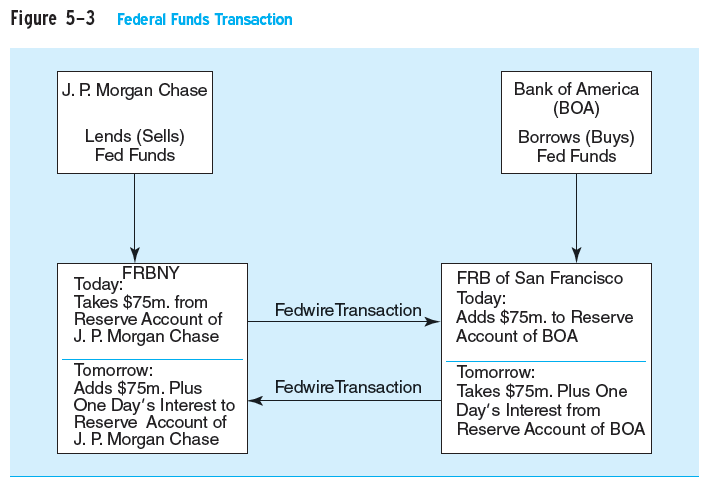
\includegraphics[height=0.37\textheight,keepaspectratio]{figures/slide22_img.png}
\end{figure}
\end{column}
\begin{column}{0.54\textwidth}
\footnotesize
\textbf{Today --- loan initiation:}
\begin{itemize}
  \item J.P.\ Morgan Chase has extra reserves; Bank of America needs more (regulatory requirements, outflows, avoiding overdrafts)
  \item J.P.\ Morgan lends (``sells'') \$75 million in fed funds to BOA --- an unsecured overnight loan; BOA repays principal + interest tomorrow
\end{itemize}
\textbf{Tomorrow --- repayment with interest:}
\begin{itemize}
  \item BOA repays \$75m principal plus one day's interest at the agreed fed funds rate
  \item Via Fedwire in reverse: FRB San Francisco debits \$75m + interest from BOA; FRBNY credits \$75m + interest to J.P.\ Morgan
  \item The lender earns interest income; the borrower pays the cost of overnight reserves
\end{itemize}
\end{column}
\end{columns}
\note{Federal funds transaction in the U.S. banking system --- an overnight, unsecured loan of reserve balances between two commercial banks.}
\end{frame}

% [src: 24]
\begin{frame}{Repurchase Agreements (Repos)}
A \textbf{repurchase agreement (repo or RP)} is the sale of a security with an agreement to buy it back at a \textbf{higher price} in the future --- essentially a short-term \textbf{collateralized} loan (typical collateral: U.S.\ Treasury securities).
\begin{itemize}
  \item The repo rate is typically \textbf{lower} than the Fed funds rate because repos are collateralized loans
  \item If collateralized by risky assets, the repo may involve a \textbf{haircut} --- e.g., to borrow \$100 the repo seller must sell securities currently worth \$102 (a \$2 haircut)
  \item A \textbf{reverse repo} is the purchase of a security with an agreement to sell it back in the future
\end{itemize}
\end{frame}

% [src: 25, 26]
\begin{frame}{Commercial Paper}
\textbf{Commercial paper (CP)} is short-term \textbf{unsecured} debt issued by corporations to fund working capital --- typically accounts receivable, inventory financing, or bridge funding.
\begin{itemize}\small
  \item Maturities of 1--270 days; total outstanding $\approx$ \$1.45 trillion (July 2026)
  \item Ratings are essential --- most CP is rated A-1/P-1 (prime) or A-2/P-2 by Moody's/S\&P
  \item Usually held to maturity; no active secondary market; yields quoted on discount yield (like T-bills)
\end{itemize}
\vspace{0.2em}
Three main types: \textbf{nonfinancial CP} (industrial companies), \textbf{financial CP} (bank holding companies, finance subsidiaries), and \textbf{asset-backed CP} (ABCP, issued by conduits backed by receivables or other assets).
\begin{center}

\includegraphics[height=0.30\textheight,keepaspectratio]{figures/slide26_img_flat.png}
\end{center}
\end{frame}

% [src: 27]
\begin{frame}{Negotiable Certificates of Deposit}
A \textbf{negotiable CD (NCD)} is a bank-issued time deposit that specifies the interest rate and maturity date.
\begin{itemize}
  \item Denominations range from \$100{,}000 to \$10 million; \$1 million is the most common
  \item Unlike standard retail CDs, NCDs have market-determined interest rates and can be liquidated before maturity by selling to another investor
  \item Often purchased by money market mutual funds with pools of funds from individual investors
\end{itemize}
\end{frame}

% [src: 28, 29]
% slide29_img.emf and slide29_img1.emf (native diagrams) converted to PNG via GDI+ — keep all files.
\begin{frame}{Banker's Acceptances}
A \textbf{banker's acceptance (BA)} is a short-term debt instrument used in \textbf{international trade finance} --- to facilitate secure payments between importers and exporters, especially when the parties do not fully trust each other or extended payment terms are needed.
\begin{itemize}\small
  \item A \textbf{time draft} (a written order to pay a specified amount at a future date) that has been ``accepted'' by a bank
  \item By accepting, the bank \textbf{unconditionally promises} to pay the face value at maturity --- replacing the importer's credit risk with the bank's (usually much stronger) credit quality
\end{itemize}
\vspace{0.2em}
\begin{center}
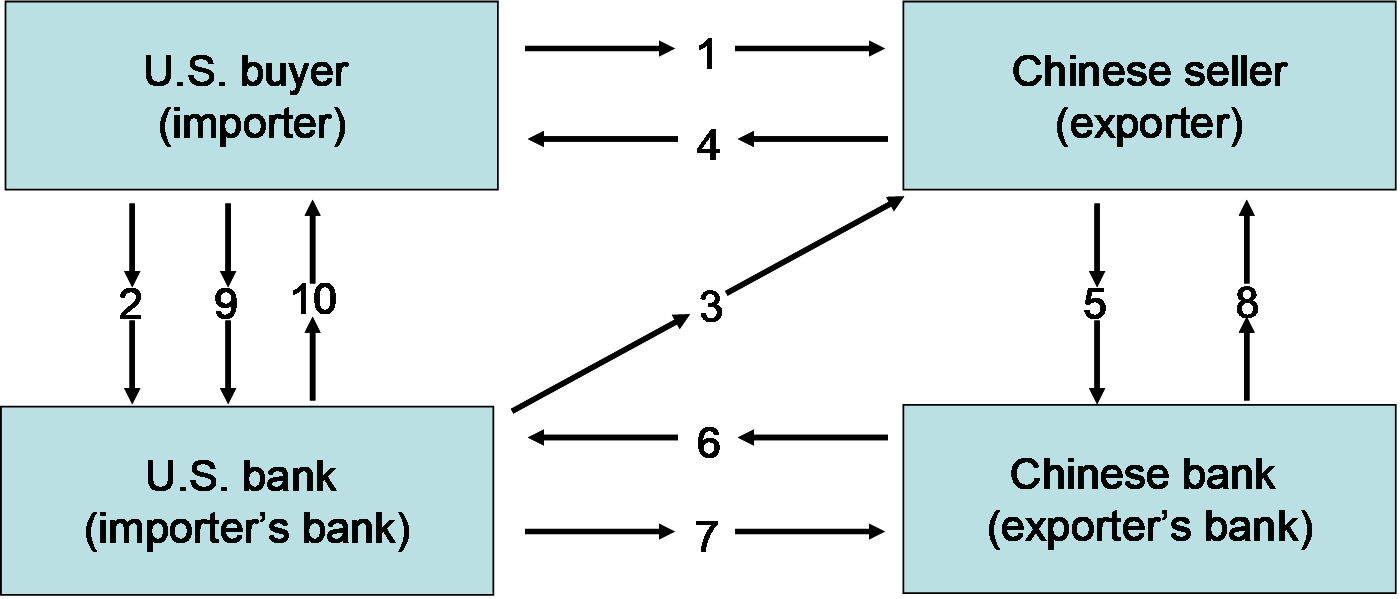
\includegraphics[height=0.26\textheight,keepaspectratio]{figures/slide29_img_flat.png}
\hspace{0.4em}
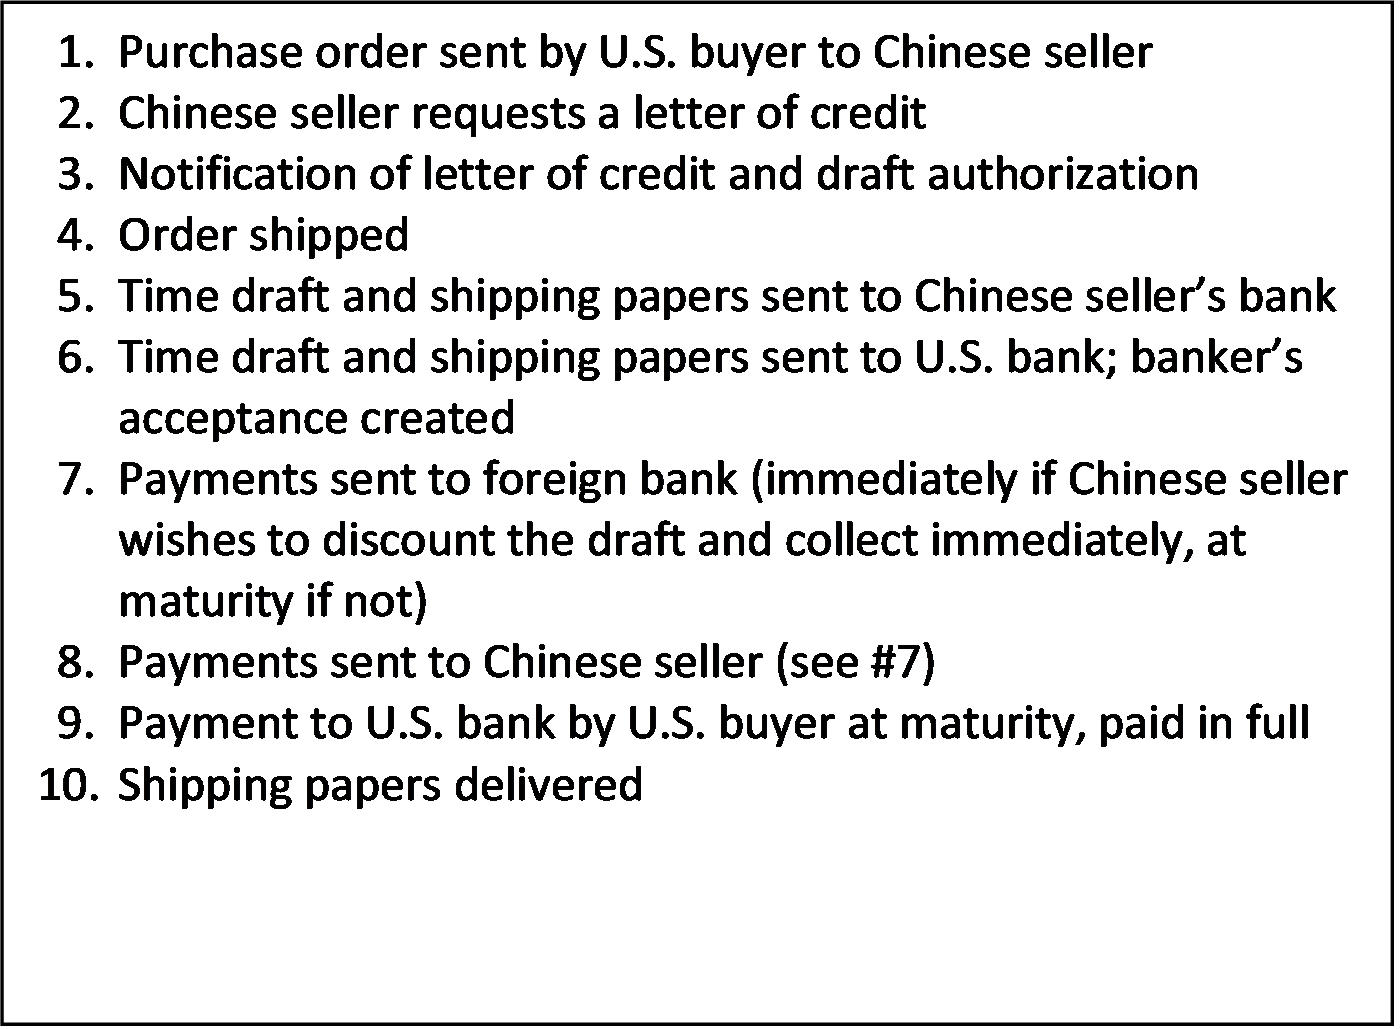
\includegraphics[height=0.26\textheight,keepaspectratio]{figures/slide29_img1_flat.png}
\end{center}
\end{frame}

% [src: 30, 31]
\begin{frame}{Why Banker's Acceptances Are Attractive}
\begin{columns}
\begin{column}{0.52\textwidth}
\begin{table}
\centering
\scriptsize
\begin{tabular}{p{0.15\textwidth}p{0.30\textwidth}}
\toprule
\textbf{Party} & \textbf{Main benefit} \\
\midrule
Exporter & Bank's payment guarantee instead of relying on unknown importer \\
Importer & Deferred payment terms (90--180 days credit) without paying upfront \\
Both & Counterparty risk significantly reduced \\
Banks & Fees for acceptance; can create highly marketable short-term paper \\
\bottomrule
\end{tabular}
\end{table}
\end{column}
\begin{column}{0.46\textwidth}
\footnotesize
BAs trade at a discount in the secondary money market and are among the \textbf{safest short-term instruments}:
\begin{itemize}
  \item Often safer than commercial paper because of the bank's unconditional guarantee
  \item Typically yield slightly more than T-bills but less than regular CP, due to low risk
  \item In short: a BA transforms a risky importer's promise into a safe, bank-guaranteed, tradable short-term credit instrument
\end{itemize}
\end{column}
\end{columns}
\end{frame}

% [src: 32]
\begin{frame}{Money Market Instruments: Summary}
\begin{table}
\centering
\small
\begin{tabular}{p{0.20\textwidth}p{0.20\textwidth}p{0.13\textwidth}p{0.34\textwidth}}
\toprule
\textbf{Instrument} & \textbf{Issuer} & \textbf{Maturity} & \textbf{Key features} \\
\midrule
Treasury bills & Government (U.S.\ Treasury) & 4 weeks--1 year & Zero-coupon, sold at discount, very safe \\
Commercial paper & Corporations & 1--270 days & Unsecured promissory notes, short-term corporate borrowing \\
Negotiable CDs & Banks & 1 month--1 year & Time deposits, often negotiable (NCDs) \\
Repos & Banks, dealers, institutions & Overnight--few weeks & Collateralized short-term loans (usually government securities) \\
Banker's acceptances & Banks (accepting trade drafts) & 30--180 days & International trade, bank-guaranteed \\
Federal funds & Banks (interbank) & Overnight & Unsecured loans between banks to meet reserve requirements \\
\bottomrule
\end{tabular}
\end{table}
\end{frame}

% [src: 33]
% Size figures refreshed 2026-09-09 from refresh_data_rates_bonds_mm.md (W4 #1--#7):
% T-bills $7.25T (MSPD, Aug 2026); triparty repo $4.4T o/s (OFR, end-2025); CP $1.45T
% (FRED DTBSPCKNMM, July 2026); NCDs ~$1.7T (SIFMA, 2024); fed funds ~$100B/day
% (NY Fed, Aug 2026); MMF $7.98T record AUM (ICI, Sept 2026). Eurodollar size has no
% current single official figure — kept as labeled order-of-magnitude estimate.
\begin{frame}{Money Market Instruments Outstanding}
\begin{table}
\centering
\scriptsize
\begin{tabular}{p{0.17\textwidth}p{0.14\textwidth}p{0.13\textwidth}p{0.26\textwidth}p{0.16\textwidth}}
\toprule
\textbf{Instrument} & \textbf{Issuer} & \textbf{Maturity} & \textbf{Key feature} & \textbf{Approx.\ size} \\
\midrule
Treasury bills & US Treasury & 4--52 weeks & Zero default risk; auctioned weekly & \$7.25T (Aug 2026) \\
Repos & Dealers, banks & Overnight--3 months & Secured by Treasuries/MBS & \$4.4T triparty o/s (end-2025) \\
Commercial paper & Corporations, banks, SPVs & 1--270 days & Unsecured (non-fin.) or asset-backed & \$1.45T (July 2026) \\
Negotiable CDs & Banks & 2 weeks--1 year & Bank liability; tradeable secondary market & $\sim$\$1.7T (SIFMA, 2024) \\
Federal funds & Banks & Overnight & Interbank reserve lending; Fed-targeted & $\sim$\$100B/day (Aug 2026) \\
Eurodollar deposits & Offshore banks & Overnight--1 year & USD outside US; no Fed regulation & Multi-\$T est.; shrank post-LIBOR \\
Money market funds & Investment companies & Daily liquid & Pooled vehicle investing in all above & \$7.98T AUM (Sept 2026) \\
\bottomrule
\end{tabular}
\end{table}
\begin{center}
\small Sources: Treasury MSPD; OFR; FRED (DTBSPCKNMM); SIFMA; NY Fed; ICI; BIS. Figures as of the dates shown; retrieved Sept 2026.
\end{center}
\end{frame}

% [src: 34]
% TODO: recreate chart — the source deck has a NATIVE CHART (money market yields vs. T-bills,
% risk spreads around crises) with no extracted figure.
\begin{frame}{The Money Market: Safe, but Not Risk-Free}
Money market instruments are \textbf{safe, but not risk-free}. Investors require higher yields on money market securities than on T-bills:
\begin{itemize}
  \item Spreads (risk premia) often increase during crisis periods
  \item Some instruments even defaulted --- e.g., commercial paper issued by Lehman Brothers became worthless in 2008
\end{itemize}
\note{CD: certificate of deposit.}
\end{frame}

% ============ INTERNATIONAL MONEY MARKETS ============

% [src: 35]
\begin{frame}{International Money Markets: Eurodollars}
\textbf{Eurodollars} are US dollar-denominated deposits held \textbf{outside the United States} --- in London, Singapore, Hong Kong, the Cayman Islands, and other offshore centers. The term ``Euro'' is historical and geographical; any offshore USD deposit qualifies.
\begin{itemize}
  \item Not subject to Federal Reserve reserve requirements or FDIC insurance --- giving offshore banks both higher flexibility and higher credit risk
  \item Historically, the rate offered for borrowing Eurodollar funds was the \textbf{London Interbank Offered Rate (LIBOR)}, which ceased in 2023; offshore USD now prices mostly off SOFR-linked benchmarks
  \item Estimated outstanding volume: on the order of \$10 trillion in deposits and loans (order-of-magnitude estimate --- the market has contracted since the LIBOR era); the linked derivatives footprint is far larger: total OTC derivatives notional was \$844.6 trillion at end-2025, of which \$669.5 trillion in interest-rate derivatives (BIS)
\end{itemize}
\end{frame}

% [src: 36]
\begin{frame}{The LIBOR-to-SOFR Transition}
One of the most consequential structural changes in money markets: the transition from USD LIBOR to SOFR as the primary short-term dollar benchmark.
\begin{description}
  \item[LIBOR] A panel-based, \emph{unsecured} rate --- an average of rates at which banks \emph{reported} they could borrow; at its pre-transition peak the reference rate for $\sim$\$350 trillion in contracts. Its fatal flaw emerged in 2012: manipulation allegations showed banks had submitted false quotes, rendering LIBOR untrustworthy. Panel LIBOR ceased on 30 June 2023; synthetic USD LIBOR ended 30 September 2024
  \item[SOFR] Administered by the Federal Reserve Bank of New York; a \emph{transaction-based}, \emph{secured} rate --- a volume-weighted median of actual overnight repo transactions collateralized by US Treasury securities
\end{description}
\note{WSJ article, 5/2/13: ``Clubby London Trading Scene Fostered Libor Rate-Fixing Scandal'' (online.wsj.com). UBS was fined \$1.52 billion, RBS \$612 million, and Barclays \$450 million.}
\end{frame}

% [src: 37]
\begin{frame}{LIBOR vs.\ SOFR}
\begin{table}
\centering
\small
\begin{tabular}{llp{0.36\textwidth}}
\toprule
\textbf{Feature} & \textbf{USD LIBOR (ceased 2023)} & \textbf{SOFR} \\
\midrule
Rate type & Unsecured & Secured (repo collateral) \\
Determination & Panel survey & Transaction-based \\
Tenor & Was overnight--12m (ceased) & Overnight (Term SOFR derived) \\
Credit risk premium & Yes (bank credit) & No (near-zero, Treasury collateral) \\
Manipulation risk & High (demonstrated) & Low (volume-based median) \\
\bottomrule
\end{tabular}
\end{table}
\end{frame}

% ============ MONEY MARKET YIELDS ============

% [src: 38]
\section{Money Market Yields}

% [src: 39, 40]
% Formula images (slide40_img.png, slide40_img1.png) replaced by native math.
\begin{frame}{Money Market Yields: Special Quoting Conventions}
Money market securities use special rate quoting conventions:
\begin{description}
  \item[Discount yield ($i_{dy}$)] Interest rate quoted on an annual basis, assuming a \textbf{360-day year}, as a percentage of \textbf{face value}:
  \[
  i_{dy} = \frac{F - P_0}{F} \times \frac{360}{n}
  \]
  \item[Single-payment yield ($i_{sp}$)] Interest rate quoted on an annual basis, assuming a \textbf{360-day year}, as a percentage of \textbf{purchase price}
\end{description}
Both may be converted to a \textbf{bond equivalent yield} ($i_{bey}$) for comparison with bonds.
\note{$i_{bey}$ is an APR. For the discount yield, note the denominator is the face value rather than the purchase price $P_0$.}
\end{frame}

% [src: 41]
% Formula images (slide41_img.png, slide41_img1.png) replaced by native math.
\begin{frame}{The Bond Equivalent Yield}
\[
i_{bey} = \frac{F - P_0}{P_0} \times \frac{365}{n}
\]
Two differences from the discount yield: the denominator is $P_0$ (purchase price) rather than face value, and the calculation uses \textbf{365} rather than 360 days.
\vspace{0.3em}
\begin{itemize}
  \item The discount yield is the \emph{quoted} rate for T-bills; the BEY is the true comparable yield for investment decisions
  \item The BEY will always be \textbf{higher} than the discount yield for the same T-bill --- it more accurately reflects the true annualized rate of return
\end{itemize}
\end{frame}

% [src: 42]
% Formula images (slide42_img.png, slide42_img1.png) replaced by native math.
\begin{frame}{Single-Payment Yields and Conversion}
Negotiable CDs and federal funds pay interest only at maturity --- quoted using \textbf{single-payment yields}:
\[
i_{sp} = \frac{F - P_0}{P_0} \times \frac{360}{n}
\qquad\Longrightarrow\qquad
i_{bey} = i_{sp} \times \frac{365}{360}
\]
Converting to a bond equivalent yield allows fair comparison of different money market instruments.
\end{frame}

% [src: 43, 44]
% Worked-solution images (slide43_img*.png, slide44_img*.png) replaced by native math;
% results match the source deck (2.038% vs. 2.028%).
\begin{frame}{Comparing Money Market Yields: Example}
A \$1M investment in 90-day commercial paper has a 2\% discount yield; an equivalent size and risk 90-day CD has a 2\% single-payment yield. \textbf{Which security offers the better return?}
\vspace{0.3em}
\begin{enumerate}
  \item \textbf{Commercial paper} ($i_{dy} = 2\%$):
  \[
  P_0 = \$1{,}000{,}000 \times \left(1 - 0.02 \times \tfrac{90}{360}\right) = \$995{,}000,
  \qquad
  i_{bey} = \frac{5{,}000}{995{,}000} \times \frac{365}{90} = 2.038\%
  \]
  \item \textbf{CD} ($i_{sp} = 2\%$):
  \[
  F = \$1{,}000{,}000 \times \left(1 + 0.02 \times \tfrac{90}{360}\right) = \$1{,}005{,}000,
  \qquad
  i_{bey} = \frac{5{,}000}{1{,}000{,}000} \times \frac{365}{90} = 2.028\%
  \]
\end{enumerate}
\textbf{The commercial paper has the better return} --- its bond equivalent yield (2.038\%) exceeds the CD's (2.028\%).
\end{frame}

% ============ MONEY MARKET FUNDS ============

% [src: 45]
\section{Money Market Funds}

% [src: 46]
\begin{frame}{Money Market Funds (MMFs)}
MMFs are \textbf{pooled investment vehicles} that invest primarily in money market securities --- T-bills, commercial paper, CDs, repos. They function as \emph{de facto} bank accounts for institutional cash. Primary objectives:
\begin{itemize}
  \item Preserve capital
  \item Provide daily liquidity
  \item Provide competitive yields to investors
  \item Maintain a stable net asset value (NAV), typically \$1 per share
\end{itemize}
\end{frame}

% [src: 47]
\begin{frame}{Size and Growth of MMFs}
\begin{figure}
\centering

\includegraphics[height=0.72\textheight,keepaspectratio]{figures/slide47_img_flat.png}
\end{figure}
\end{frame}

% [src: 48, 49]
\begin{frame}{MMF Types and Structures}
\begin{description}
  \item[Government MMFs] Invest $\geq$99.5\% in US government securities, repo collateralized by government securities, and cash; must maintain a stable \$1.00 NAV for all investor classes
  \item[Prime MMFs] Invest in any money market instrument including CP, CDs, and repo; retail prime funds maintain stable NAV, institutional prime funds must use floating NAV
  \item[Tax-exempt/municipal MMFs] Invest in short-term municipal paper; income is federally tax-free
\end{description}
\vspace{0.3em}
\begin{center}

\includegraphics[height=0.34\textheight,keepaspectratio]{figures/slide49_img_flat.png}
\end{center}
\end{frame}

% [src: 50]
\begin{frame}{MMF Types: Government vs.\ Prime}
\begin{table}
\centering
\small
\begin{tabular}{p{0.12\textwidth}p{0.33\textwidth}p{0.31\textwidth}p{0.12\textwidth}}
\toprule
\textbf{Type} & \textbf{Primary investments} & \textbf{Key features} & \textbf{Typical investors} \\
\midrule
Government & U.S.\ Treasury securities, agency debt, and repos backed by government securities (at least 99.5\% government assets for Treasury-only funds) & Lowest risk; exempt from certain liquidity fee rules; stable NAV; taxable income; yields tied to the Fed funds rate & Risk-averse investors seeking safety \\
Prime & Corporate commercial paper, bank CDs, and some government securities & Higher yields than government funds but slightly more credit risk; may include floating NAV for institutional class & Investors balancing yield and safety \\
\bottomrule
\end{tabular}
\end{table}
\end{frame}

% [src: 51]
\begin{frame}{Money Market Fund Rates vs.\ Bank Deposit Rates}
\textbf{Why would anyone want to put their money in a bank account?}
\begin{figure}
\centering
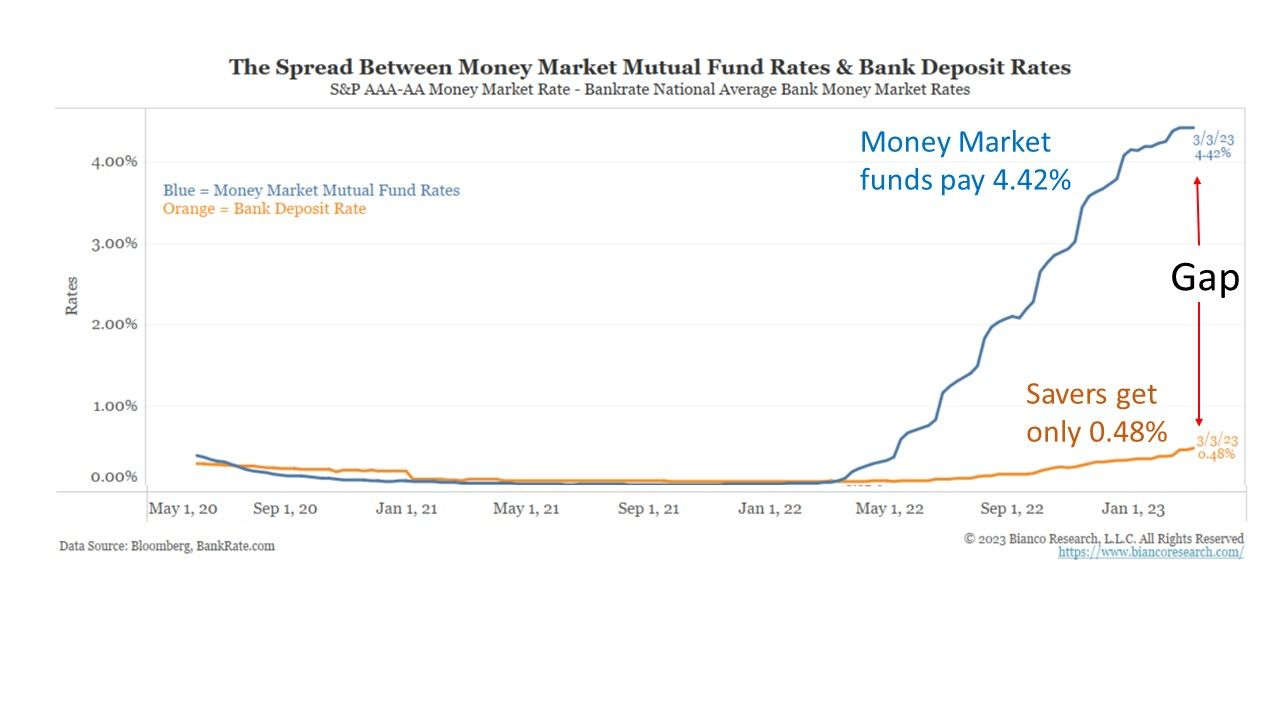
\includegraphics[height=0.60\textheight,keepaspectratio]{figures/slide51_img.jpg}
\end{figure}
\end{frame}

% [src: 52, 53]
\begin{frame}{MMF Regulation and Yields}
\begin{columns}
\begin{column}{0.48\textwidth}
\textbf{SEC Rule 2a-7} (Investment Company Act of 1940) governs all US MMFs:
\begin{itemize}\footnotesize
  \item Portfolio maturity limits: WAM $\leq$ 60 days; WAL $\leq$ 120 days
  \item Credit quality: only ``eligible securities'' rated A-1/P-1 or equivalent
  \item Diversification: no single issuer $>$ 5\% (except government securities)
  \item Liquidity minimums (effective April 2024): daily $\geq$ 25\%; weekly $\geq$ 50\%
  \item October 2024: mandatory liquidity fees on institutional prime/tax-exempt funds; discretionary redemption gates removed --- prime funds now hold only $\sim$16\% of MMF assets (vs.\ $\sim$28\% pre-reform)
  \item Reporting: monthly Form N-MFP to the SEC, publicly available
\end{itemize}
\end{column}
\begin{column}{0.48\textwidth}
\textbf{MMF yields} respond almost mechanically to the fed funds rate --- portfolio maturities are so short (WAM typically 30--45 days) that most holdings reprice within weeks:
\[
\text{MMF yield} \approx \text{EFFR} - \text{expenses} \pm \alpha
\]
\begin{itemize}\small
  \item Government MMFs track the Fed funds rate minus management fees ($\sim$10--15 bps)
  \item Prime MMFs earn a spread above government MMFs ($\sim$10--30 bps) by accepting CP and CD credit exposure
\end{itemize}
\end{column}
\end{columns}
\end{frame}

% [src: 54, 55]
% CJK characters (余额宝) omitted — the course theme has no CJK font support under pdfLaTeX.
\begin{frame}{MMFs in China: Yu'e Bao}
\textbf{Yu'e Bao} is a hugely popular money market fund offered through Alipay, managed primarily by Tianhong Asset Management.
\begin{itemize}\small
  \item Launched 2013; lets users invest idle cash (``leftover'' change from transactions) in a low-risk MMF
  \item The world's largest money market fund around 2017--2019; at its peak (Q1 2018) over ¥1.69 trillion ($\sim$\$260--268 billion) AUM, surpassing major US funds like JPMorgan's US Government Money Market Fund
  \item Growth driven by convenience, competitive yields, and Alipay's massive user base --- then a long decline: by end-June 2026 AUM was down to $\sim$¥680 billion ($\sim$\$94 billion), roughly 60\% below peak, with the 7-day annualized yield below 1\% since May 2026 (vs.\ 6--7\% in its early years)
  \item From 2017--2018 Chinese regulators curbed risks: subscription caps for individuals (later relaxed), requirements for more liquid assets and reduced lower-quality exposure, plus competition from bank wealth products --- it was overtaken by US institutional funds from JPMorgan and Fidelity; falling Chinese money-market yields then compressed both its size and its appeal
\end{itemize}
\end{frame}

% [src: 56]
\begin{frame}{MMFs: What Are the Risks?}
MMFs aim for low volatility and are among the safest investments --- but not entirely risk-free:
\begin{description}
  \item[Interest rate risk] Yields fall with declining rates, potentially underperforming inflation
  \item[Credit risk] Minimal but possible if issuers default
  \item[Liquidity risk] In market stress, funds may face redemption pressures, leading to forced sales at losses
  \item[No government insurance] Unlike bank deposits, no FDIC protection; SIPC covers only brokerage failures
  \item[Opportunity cost] Lower returns than stocks or longer-term bonds
\end{description}
\end{frame}

% [src: 57, 58]
\begin{frame}{Mini Case: The 2008 GFC and the Reserve Primary Fund}
The 2008 crisis highlighted MMF vulnerabilities when the Reserve Primary Fund \textbf{``broke the buck.''}
\begin{columns}
\begin{column}{0.56\textwidth}
\begin{itemize}\small
  \item After Lehman Brothers' bankruptcy on September 15, the fund faced a massive wave of redemptions (a ``run'')
  \item On September 16 it wrote its Lehman holdings down to zero; NAV fell from the stable \$1.00 to \textbf{\$0.97} --- only the second time in history a MMF broke the buck
  \item The fund suspended redemptions for orderly liquidation; investors eventually recovered $\approx$99.1 cents on the dollar, but the final distribution did not occur until \textbf{December 2014}, leaving capital frozen for years
\end{itemize}
\end{column}
\begin{column}{0.42\textwidth}
\begin{figure}
\centering
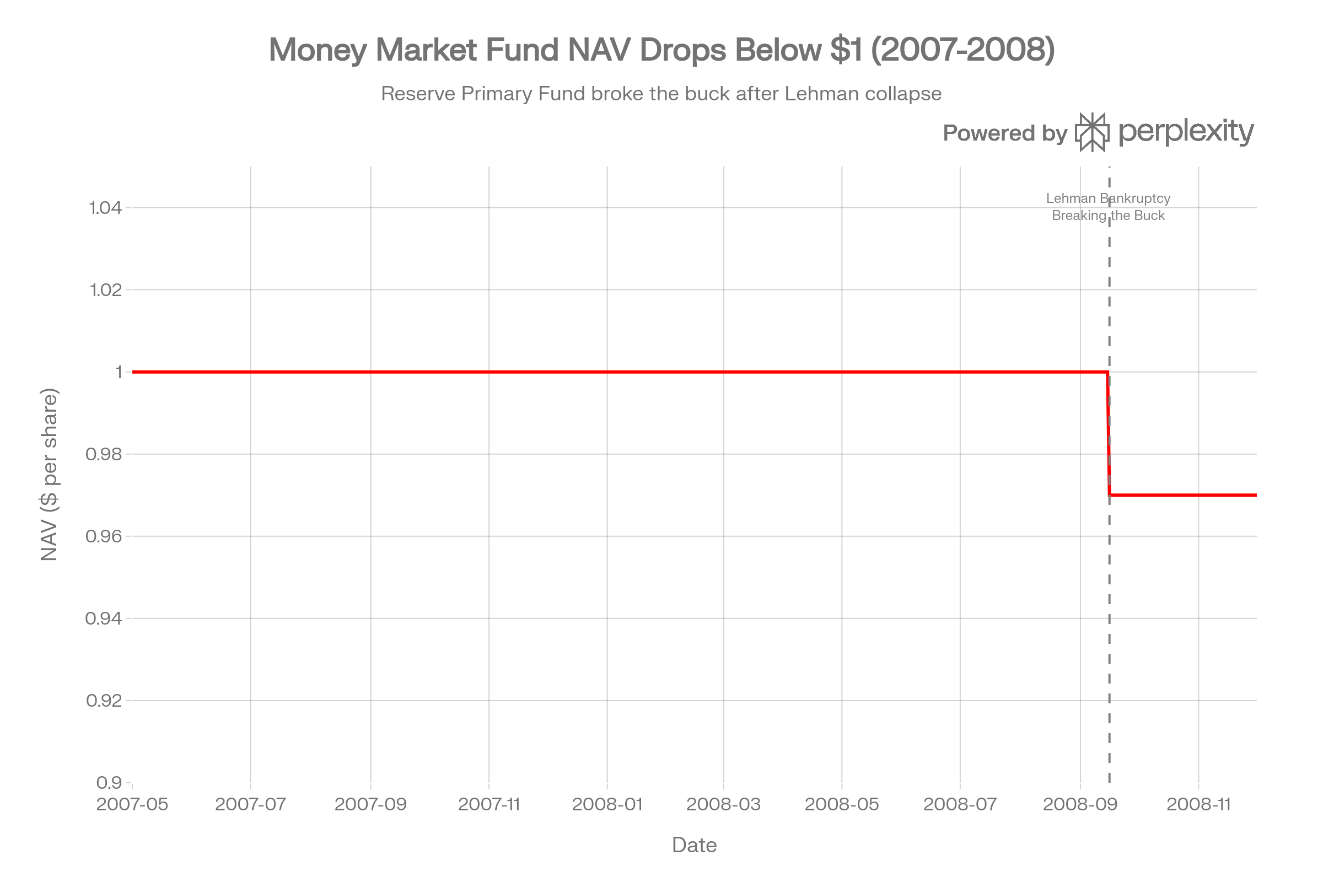
\includegraphics[height=0.48\textheight,keepaspectratio]{figures/slide58_img_flat.png}
\end{figure}
\end{column}
\end{columns}
\end{frame}

% [src: 59, 60]
\begin{frame}{Key Takeaways}
\begin{itemize}
  \item \textbf{Money market:} short-term ($\leq$ 1 year), highly liquid, low-risk securities; purpose is managing short-term funding needs and investing excess cash safely, not long-term growth
  \item \textbf{Instruments:} T-bills (default-risk free, sold at discount); fed funds (overnight unsecured interbank loans; the Fed funds rate is the policy target); repos (collateralized by Treasuries; rate $<$ Fed funds); CP (unsecured corporate debt, limited secondary market); negotiable CDs (bank time deposits, tradable); BAs (bank-guaranteed trade finance, low risk)
  \item \textbf{Yields:} special quoting conventions (discount yield, single-payment yield); the bond equivalent yield standardizes yields for comparison with bonds
  \item \textbf{MMFs:} mutual funds investing in money market securities; goals --- preserve capital, provide liquidity, maintain stable \$1.00 NAV. Not risk-free: ``breaking the buck'' in 2008, no FDIC insurance, interest rate and credit risk
\end{itemize}
\end{frame}

\end{document}
